\chapter{設計と実装}
\label{chap:implementation}
\section{1人麻雀の実装}
提案手法で提示した、期待和了平均順目の評価によるモンテカルロ木探索を評価するために、1人麻雀プレイヤーを実装した。
1人麻雀プレイヤーとは、相手プレイヤーを考えない多人数性を排除した麻雀のことである。ルールについては次の節で詳しく説明している。
本研究で実装した1人麻雀プレイヤーのフローチャート図を図\ref{1flow}に示す。

\begin{figure}[H]
 \centering
 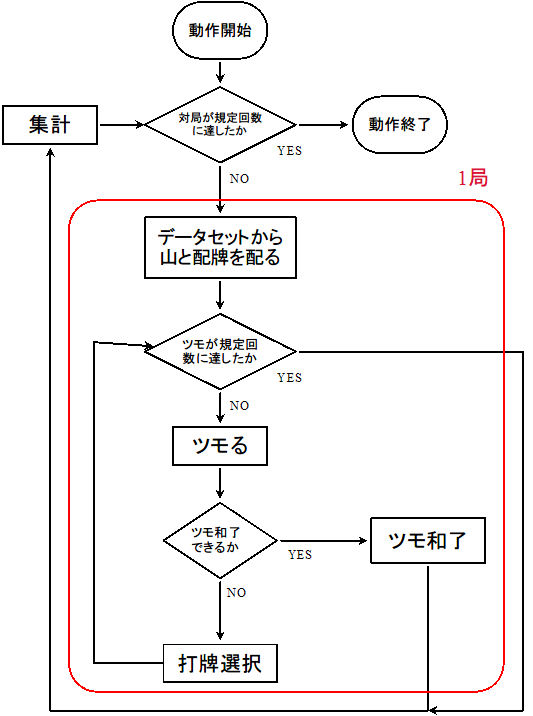
\includegraphics[keepaspectratio, scale=0.7,bb=0 0 440 540]
      {img/1flow.png}
 \caption{1人麻雀のフローチャート}
 \label{1flow}
\end{figure}

まず、1人麻雀プレイヤーにおいて開局から、終局まで行う対局のループを定義する。
開局時には、山と配牌を設置する。その後山から一つ牌をツモり、一つ捨てる動作を繰り返す。終了条件を満たした時点で終局となり、その局の成績を集計する。このループを1人麻雀プレイヤーにおける1対局と定義する。この対局のループを十分な回数行い、和了率を測定する。

% 期待和了平均順目をn順先の変化まで評価することによって性能が変わる可能性があるので、1順、2順、3順までの変化を考慮するものをそれぞれ分けて実験した。
% それぞれに対して100局のテストデータと10,000局のテストデータを与え、あがることができた局数を計測した。テストデータとは、全ての牌をランダムに並べたものを100セット用意したデータである。このデータから 13 牌を初期牌として 与え, その後牌を引いて切る動作を 27 回行い, その中であ がれたかどうかを確認した。100 局のテストデータで人間 のプレイヤとの比較を行い, 10,000 局のテストデータで各 手法の性能の評価を行った。



\subsection{1人麻雀のルール}
通常の4人麻雀では、多人数製の問題があるため、分岐や考慮すべき問題が多い難しさがある。この難しさを解消するために、相手を考慮しない1人麻雀を考える。
この1人麻雀のルールは、相手プレイヤーを考えないため、点数を支払う事による放銃や被ツモ失点などを考えない。また、相手プレイヤーによる捨て牌が存在しないので、鳴きや栄和を考えない。リーチについても、和了率の観点では不要なため、考えない。門前でツモを繰り返し行うだけのシンプルなシステムである。
% 先行研究\cite{zentsu}評価を合わせるため、ツモの回数は27回とした。

\begin{table}[htbp]
  \caption{本研究の1人麻雀プレイヤのルール}
  \label{tb:bakuuti_score}
  \begin{center}
  \begin{tabular}{c|c|c}
    \hline
    アクション  & 4人麻雀 & 1人麻雀 \\\hline\hline
    和了  & ツモ和了、ロン和了どちらも可 & ツモ和了のみ\\\hline
    点数 & 失点や和了の点数を考慮する & 点数は考えない\\\hline
    リーチ & 可能 & なし\\\hline
    鳴き & チー、ポン、カンが可能 & なし\\\hline
    終局 & 誰かが和了するか、ツモ山70枚がなくなるまで(136-14-13*4) & 和了するか、27回ツモるか\\\hline
  \end{tabular}\end{center}
\end{table}

また1人麻雀の成績の評価においてはその点数の推移よりも、和了率自体が重要だと考えられている。したがって、点数という複雑なパラメータを省いた和了率に注目したルールとなっている。その理由としては、以下のような理由が述べられる。

4人麻雀では平均順位の低いプレイヤーほど、平均和了点低く、和了率が高いことというデーターが存在する。\cite{kagaku}。したがって強いプレイヤーは点数よりも和了率を重視して打っていることがわかる。
上手いプレイヤーは手役を無理に狙わないため、平均和了点が低くなると考えられる。また麻雀の点数の特性上、満貫までの点数は指数関数的にその得点が増えていくが、満貫以上の場合は線形に近くなる。したがって、難易度に対して望める点数が割に合わない高い和了を狙うより、比較的低い点数で゙多く和了することが効率が良い。
また、失点の観点からも、4人麻雀では自分が放銃をしない場合も他プレイヤーの和了によって被ツモ失点を被ることがある。これに対しても、和了すれば他プレイヤーが和了することができないため、相手の和了を防ぐという意味でも和了率の高さは重要である。

\subsection{終了条件}
図\ref{1flow}に示した1局の終了条件は、ツモが規定回数に達するか、和了したかのいずれかとしている。4人麻雀においても、いずれかのプレイヤーが和了しない場合において、ツモの回数が規定回数(厳密には山がなくなるまでだが)に達した場合は終了となる。したがって、1人麻雀においても、和了が発生しない場合においても対局が終了するような条件を入れた。また、通常の4人麻雀ではツモの回数は、流局した場合平均的に18回である。しかし1人麻雀を評価として利用している関連研究の多く\cite{zentsu}\cite{bakuuti2013}が、1人麻雀のツモの規定回数を27回としているため、本研究でもツモの回数を27回とした。また、対局数に関しては、5000局のものと100局のもので分けた。詳しくは次章の評価で述べるが、AIアルゴリズム同士では十分な回数行い、人間プレイヤーも評価に加える際は実現が可能な100局という対局数を用いた。

\subsection{データセット}
1人麻雀でAIや人間が対局を行うとき、山や配牌は毎回ランダムに生成するわけではなく、予め用意したデータセットを扱う。1人麻雀の一局において扱う牌の数は、初期配牌13牌と山27牌の合計40牌である。この40牌を、予め麻雀の対局で使用可能な136牌の中から、ランダムに抽出し並べておく。このセットを対局数分用意したものがデータセットである。このように同じデータセットで十分な回数それぞれの手法で1人麻雀を打つことで、手法ごとの和了率の優劣が精密に比較可能である。

% \subsection{打牌選択}
% ・どのような手法を選択したか
% 爆打モンテカルロ法
% UCB1モンテカルロ法
% LinUCBを用いた方法
% ・どのように実装したか どのような制限を加えたか
% (プレイアウトの回数、CPUや実装コード)
% 計算量の問題


% \subsection{期待平均和了順目の探索の深さの評価}
% \subsection{モンテカルロ法の探索領域}


\section{4人麻雀の自動打ちシステムの実装} %麻雀サーバーとの対戦
本研究の提案手法のアルゴリズムが4人麻雀でも有用かどうかを調べるために、4人麻雀で実際に対戦するための自動打ちシステムを実装した。言語はC\#を用い、ビルド環境はVisualStudio 2015 Communityを用いた。このシステムを動かす場所として、オンライン麻雀サイト「天鳳」を選んだ。実装した自動打ちシステムの大きな流れを図\ref{imp1}に示す。

% 本研究では1人麻雀における和了率の向上を目指すため、和了率の数理的評価とモンテカルロ法を適用する部分を限定する手法をとった。佐藤らは、1人麻雀における和了率を有効牌を数え上げて大きくなるようにすることで、和了率の最大化を図り、これを4人麻雀で打たせレートを取った。同じように本研究手法でも4人麻雀で打たせた結果を比較した。

\begin{figure}[h]
 \centering
 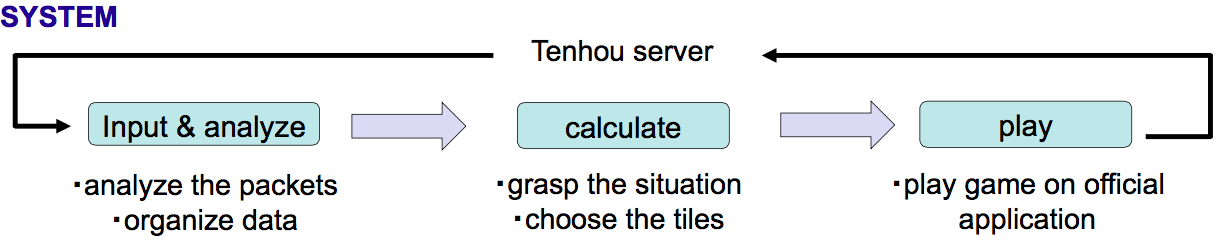
\includegraphics[keepaspectratio, scale=0.4
 ,bb=0 0 1226 243]
      {img/imp1.png}
 \caption{天鳳上で自動打ちするためのシステムの設計図}
 \label{imp1}
\end{figure}

まず、天鳳サーバーから受け取った情報を送られてくるパケットとして読み取る。次に、受け取った情報を整理・計算し選択する打牌を決定する。最後に、決定した打牌を公式アプリケーションを通じて天鳳サーバーにまた送るといった流れである。次の節以降その詳細について解説する。

\subsection{オンライン麻雀サイト天鳳}
天鳳は、現在インターネット上で麻雀を打つことができるサイトの中で最も利用者が多いサイトであり、登録者は390万人を超える大型のサイトである。また、アクティブユーザー(180日以内の対戦履歴があるプレーヤ数)は27万人を超え、現在最も活気のあるインターネット上の麻雀フィールドである。天鳳では麻雀研究に対する支援が充実しているという面も大きい。
最高ランク者のみが打つことのできる鳳凰卓というクラスの試合データ(以下牌譜)を全て公開しており、より良質な強者の牌譜を取得することができる。これらの牌譜は一日に約500試合ほど手に入り、量ともに十分利用できる。これについては、筆者も強者の統計的な手順について研究する際によく利用させていただいた。また、天鳳ではAIで麻雀を打つことを一定の条件下で許可している点も大きい。鳳凰卓については人間同士の生粋の強者のフィールドというコンセプトがあるため許可されていないが、その下の特上卓以下では条件を揃えることで対戦することが可能である。
一番下の一般卓については、最も低ランクなため対戦人数も多いため、AIによる影響が少ないと考えられている。そのためある程度対戦が可能なAIであれば、他プレイヤーの迷惑にならないような範囲での利用が許可されている。また、一般卓と鳳凰卓の間の上級卓・特上卓では、AIを用いて他のプレイヤーの不正検出に協力するという条件を元にAIの稼働を許可されている。AIを稼働させることによる他プレイヤーのメリットを提供することで、反対するものが少なくなるからである。本研究のシステムは、一般卓で稼働させた。

\begin{table}[h]
  \caption{ランク別リスト・AI稼働条件}
  \label{tb:rate2231}
  \begin{center}
  \begin{tabular}{c|c|c|c|c}
    \hline
    卓 & 一般卓   & 上級卓 & 特上卓 & 鳳凰卓\\\hline\hline
    レベル & 下位約80\% & 上位約20\% & 上位約10\% & 上位約1\% \\\hline
    AI稼働条件 & マナー厳守 & 不正検出に協力 & 不正検出に協力 & 不可\\\hline
  \end{tabular}\end{center}
\end{table}

% \subsection{プレイさせた天鳳のルール}
% ・ルールフロー図
% ・・天鳳上の制約(ルール)
% ・天鳳上の制約(マシン上の問題 持ち時間)

\subsection{入力}
天鳳サーバーから送られてくる情報を読み取るためには、プレイするための公式アプリケーションを扱う必要がある。天鳳では未だにAIを動かすための公式APIが公開されていないので、公式アプリケーションでプレイした情報を画像認識して解析するか、送られてくるパケットを解析する必要がある。本研究では、kmo2氏が公開している天鳳パケット解析用オープンソース\cite{kmo2}を利用し、パケット解析を利用することで情報の入力を行った。

\subsection{計算}
・天鳳からの情報をどういうふうな構造体で保存しているかどうかとか。

% \begin{figure}[h]
%  \centering
%  \includegraphics[keepaspectratio, scale=0.1,bb=0 0 3024 4032]
%       {img/flow.jpg}
%  \caption{4人麻雀自動打ちシステムのフローチャート}
% \end{figure}

また、シャンテン数の計算方法については、バックトラック法を用いた。バックトラック法とは、8クイーン問題の解決法で良くあげられるように、難しい組み合わせの問題を効率よく解くために考案された方法である。麻雀においては、シャンテン数を求めることはすなわち決められた牌姿を要素ごとの組み合わせに分解することであり、バックトラック法が有用である。雀頭・メンツ・ターツの組み合わせを最もシャンテン数を下げる形で分解することが必要になる。麻雀の和了形においては、雀頭が一つであるため、まずは雀頭として考えられる要素を取り出す。次に、メンツとして考えられる要素を取り出し、最後にターツを取り出す。メンツはターツからシャンテン数を一つ下げた形であるため、メンツで取り出せる部分がある場合はそちらを優先して行う。このようにして各要素の優先順位を付けながら考えられる組み合わせを抽出したとき、最もシャンテン数が小さいものがその牌姿のシャンテン数である。

\begin{figure}[h]
 \centering
 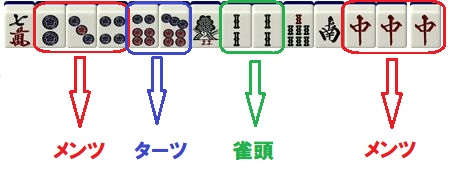
\includegraphics[keepaspectratio, scale=1,bb=0 0 320 220]
      {img/back.jpg}
 \caption{シャンテン数を求めるバックトラック法}
 \label{zu}
\end{figure}

\subsection{出力}
計算過程によって決定した牌を、天鳳サーバーに送信するためにも、プレイ用の公式アプリケーションを用いる。公式アプリケーションを介さないで直接データを送ることは、少しでも不正なプレイにならないようにするために必要なことである。公式アプリケーションで打牌を行うためには、決定した打牌をGUIで操作して選択する必要がある。したがって、出力過程では選択した牌をクリックできるよう、マウスイベントを呼ぶプログラム実装した。天鳳において公式アプリケーションで自動理牌を行うと、マンズ、ピンズ、ソーズ、字牌の順番になる。そのため、手牌の情報から切りたい牌が手牌の左から何番目にあるかを計算することができる。これを利用して、予め手牌の左端の座標を記憶し、そこから切りたい牌がどれだけ右側にあるかを計算させて、擬似的に切りたい牌を切るように設計した。


